% -*- Mode:TeX -*-

%% IMPORTANT: The official thesis specifications are available at:
%%            http://libraries.mit.edu/archives/thesis-specs/
%%
%%            Please verify your thesis' formatting and copyright
%%            assignment before submission.  If you notice any
%%            discrepancies between these templates and the 
%%            MIT Libraries' specs, please let us know
%%            by e-mailing thesis@mit.edu

%% The documentclass options along with the pagestyle can be used to generate
%% a technical report, a draft copy, or a regular thesis.  You may need to
%% re-specify the pagestyle after you \include  cover.tex.  For more
%% information, see the first few lines of mitthesis.cls. 

%\documentclass[12pt,vi,twoside]{mitthesis}
%%
%%  If you want your thesis copyright to you instead of MIT, use the
%%  ``vi'' option, as above.
%%
%\documentclass[12pt,twoside,leftblank]{mitthesis}
%%
%% If you want blank pages before new chapters to be labelled ``This
%% Page Intentionally Left Blank'', use the ``leftblank'' option, as
%% above. 

\documentclass[12pt,twoside]{mitthesis}
\usepackage{lgrind}
%% These have been added at the request of the MIT Libraries, because
%% some PDF conversions mess up the ligatures.  -LB, 1/22/2014
\usepackage{cmap}
\usepackage{float}
\usepackage{graphicx}
\usepackage{caption} \captionsetup[table]{singlelinecheck=false}
\usepackage[font=footnotesize]{caption}
\usepackage[T1]{fontenc}
\usepackage{todo}
\pagestyle{plain}
\raggedbottom

%% This bit allows you to either specify only the files which you wish to
%% process, or `all' to process all files which you \include.
%% Krishna Sethuraman (1990).

%\typein [\files]{chap1}
\def\files{all}
\def\all{all}
\ifx\files\all \typeout{Including all files.} \else \typeout{Including only \files.} \includeonly{\files} \fi

\begin{document}

% -*-latex-*-
% 
% For questions, comments, concerns or complaints:
% thesis@mit.edu
% 
%
% $Log: cover.tex,v $
% Revision 1.8  2008/05/13 15:02:15  jdreed
% Degree month is June, not May.  Added note about prevdegrees.
% Arthur Smith's title updated
%
% Revision 1.7  2001/02/08 18:53:16  boojum
% changed some \newpages to \cleardoublepages
%
% Revision 1.6  1999/10/21 14:49:31  boojum
% changed comment referring to documentstyle
%
% Revision 1.5  1999/10/21 14:39:04  boojum
% *** empty log message ***
%
% Revision 1.4  1997/04/18  17:54:10  othomas
% added page numbers on abstract and cover, and made 1 abstract
% page the default rather than 2.  (anne hunter tells me this
% is the new institute standard.)
%
% Revision 1.4  1997/04/18  17:54:10  othomas
% added page numbers on abstract and cover, and made 1 abstract
% page the default rather than 2.  (anne hunter tells me this
% is the new institute standard.)
%
% Revision 1.3  93/05/17  17:06:29  starflt
% Added acknowledgements section (suggested by tompalka)
% 
% Revision 1.2  92/04/22  13:13:13  epeisach
% Fixes for 1991 course 6 requirements
% Phrase "and to grant others the right to do so" has been added to 
% permission clause
% Second copy of abstract is not counted as separate pages so numbering works
% out
% 
% Revision 1.1  92/04/22  13:08:20  epeisach

% NOTE:
% These templates make an effort to conform to the MIT Thesis specifications,
% however the specifications can change.  We recommend that you verify the
% layout of your title page with your thesis advisor and/or the MIT 
% Libraries before printing your final copy.
\title{Negotiation Strategies in American-North Korean Nuclear Talks, 1992-2013}

\author{Haley Brandt-Erichsen}
% If you wish to list your previous degrees on the cover page, use the 
% previous degrees command:
%       \prevdegrees{A.A., Harvard University (1985)}
% You can use the \\ command to list multiple previous degrees
%       \prevdegrees{B.S., University of California (1978) \\
%                    S.M., Massachusetts Institute of Technology (1981)}
\department{Department of Nuclear Science and Engineering}

% If the thesis is for two degrees simultaneously, list them both
% separated by \and like this:
% \degree{Doctor of Philosophy \and Master of Science}
\degree{Bachelor of Science in Nuclear Science and Engineering}

% As of the 2007-08 academic year, valid degree months are September, 
% February, or June.  The default is June.
\degreemonth{June}
\degreeyear{2016}
\thesisdate{May 6, 2016}

%% By default, the thesis will be copyrighted to MIT.  If you need to copyright
%% the thesis to yourself, just specify the `vi' documentclass option.  If for
%% some reason you want to exactly specify the copyright notice text, you can
%% use the \copyrightnoticetext command.  
%\copyrightnoticetext{\copyright IBM, 1990.  Do not open till Xmas.}

% If there is more than one supervisor, use the \supervisor command
% once for each.
\supervisor{R. Scott Kemp}{Assistant Professor}

% This is the department committee chairman, not the thesis committee
% chairman.  You should replace this with your Department's Committee
% Chairman.
\chairman{Michael P. Short}{Chairman, NSE Committee for Undergraduate Students}

% Make the titlepage based on the above information.  If you need
% something special and can't use the standard form, you can specify
% the exact text of the titlepage yourself.  Put it in a titlepage
% environment and leave blank lines where you want vertical space.
% The spaces will be adjusted to fill the entire page.  The dotted
% lines for the signatures are made with the \signature command.
\maketitle

% The abstractpage environment sets up everything on the page except
% the text itself.  The title and other header material are put at the
% top of the page, and the supervisors are listed at the bottom.  A
% new page is begun both before and after.  Of course, an abstract may
% be more than one page itself.  If you need more control over the
% format of the page, you can use the abstract environment, which puts
% the word "Abstract" at the beginning and single spaces its text.

%% You can either \input (*not* \include) your abstract file, or you can put
%% the text of the abstract directly between the \begin{abstractpage} and
%% \end{abstractpage} commands.

% First copy: start a new page, and save the page number.
\cleardoublepage
% Uncomment the next line if you do NOT want a page number on your
% abstract and acknowledgments pages.
% \pagestyle{empty}
\setcounter{savepage}{\thepage}
%\begin{abstractpage}
%% $Log: abstract.tex,v $
% Revision 1.1  93/05/14  14:56:25  starflt
% Initial revision
% 
% Revision 1.1  90/05/04  10:41:01  lwvanels
% Initial revision
% 
%
%% The text of your abstract and nothing else (other than comments) goes here.
%% It will be single-spaced and the rest of the text that is supposed to go on
%% the abstract page will be generated by the abstractpage environment.  This
%% file should be \input (not \include 'd) from cover.tex.

\begin{center}
NEGOTIATION STRATEGIES IN AMERICAN-NORTH KOREAN NUCLEAR TALKS, 1992-2013

{\centering{By}}

{\centering{Haley Brandt-Erichsen}}

{\centering{Submitted to the Department of Nuclear Science and Engineering on May 4, 2016 In Partial Fulfillment of the Requirements for the Degree of Bachelor of Science in Nuclear Science and Engineering}}
\end{center}

\begin{flushleft}ABSTRACT

North Korea's relationship with nuclear technology has concerned the world for decades. A wide array of negotiation methods from punitive sanctions to energy assistance have been attempted to dissuade the nation from developing its weapons program---but every resolution has been temporary at best. We focus on the United States' negotiation strategy and attempt to uncover inconsistencies between it and the material facts of the North Korean situation. The historical record of past negotiations and rhetoric used by each party during previous attempts are considered in our analysis, in order to construct a picture of diplomatic evolution over time. We believe that the North Korean bargaining position---which has been highly consistent across decades of cyclic negotiating behavior---is fundamentally incompatible with US demands for complete denuclearization.

\vfill

Thesis Supervisor: R. Scott Kemp

Title: Norman C. Rasmussen Assistant Professor of Nuclear Science and Engineering\end{flushleft}


%\end{abstractpage}

% Additional copy: start a new page, and reset the page number.  This way,
% the second copy of the abstract is not counted as separate pages.
% Uncomment the next 6 lines if you need two copies of the abstract
% page.
% \setcounter{page}{\thesavepage}
% \begin{abstractpage}
% % $Log: abstract.tex,v $
% Revision 1.1  93/05/14  14:56:25  starflt
% Initial revision
% 
% Revision 1.1  90/05/04  10:41:01  lwvanels
% Initial revision
% 
%
%% The text of your abstract and nothing else (other than comments) goes here.
%% It will be single-spaced and the rest of the text that is supposed to go on
%% the abstract page will be generated by the abstractpage environment.  This
%% file should be \input (not \include 'd) from cover.tex.

\begin{center}
NEGOTIATION STRATEGIES IN AMERICAN-NORTH KOREAN NUCLEAR TALKS, 1992-2013

{\centering{By}}

{\centering{Haley Brandt-Erichsen}}

{\centering{Submitted to the Department of Nuclear Science and Engineering on May 4, 2016 In Partial Fulfillment of the Requirements for the Degree of Bachelor of Science in Nuclear Science and Engineering}}
\end{center}

\begin{flushleft}ABSTRACT

North Korea's relationship with nuclear technology has concerned the world for decades. A wide array of negotiation methods from punitive sanctions to energy assistance have been attempted to dissuade the nation from developing its weapons program---but every resolution has been temporary at best. We focus on the United States' negotiation strategy and attempt to uncover inconsistencies between it and the material facts of the North Korean situation. The historical record of past negotiations and rhetoric used by each party during previous attempts are considered in our analysis, in order to construct a picture of diplomatic evolution over time. We believe that the North Korean bargaining position---which has been highly consistent across decades of cyclic negotiating behavior---is fundamentally incompatible with US demands for complete denuclearization.

\vfill

Thesis Supervisor: R. Scott Kemp

Title: Norman C. Rasmussen Assistant Professor of Nuclear Science and Engineering\end{flushleft}


% \end{abstractpage}

\cleardoublepage

%\section*{Acknowledgments}


%%%%%%%%%%%%%%%%%%%%%%%%%%%%%%%%%%%%%%%%%%%%%%%%%%%%%%%%%%%%%%%%%%%%%%
% -*-latex-*-

% Some departments (e.g. 5) require an additional signature page.  See
% signature.tex for more information and uncomment the following line if
% applicable.
% % -*- Mode:TeX -*-
%
% Some departments (e.g. Chemistry) require an additional cover page
% with signatures of the thesis committee.  Please check with your
% thesis advisor or other appropriate person to determine if such a 
% page is required for your thesis.  
%
% If you choose not to use the "titlepage" environment, a \newpage
% commands, and several \vspace{\fill} commands may be necessary to
% achieve the required spacing.  The \signature command is defined in
% the "mitthesis" class
%
% The following sample appears courtesy of Ben Kaduk <kaduk@mit.edu> and
% was used in his June 2012 doctoral thesis in Chemistry. 

\begin{titlepage}
\begin{large}
This doctoral thesis has been examined by a Committee of the Department
of Chemistry as follows:

\signature{Professor Jianshu Cao}{Chairman, Thesis Committee \\
   Professor of Chemistry}

\signature{Professor Troy Van Voorhis}{Thesis Supervisor \\
   Associate Professor of Chemistry}

\signature{Professor Robert W. Field}{Member, Thesis Committee \\
   Haslam and Dewey Professor of Chemistry}
\end{large}
\end{titlepage}


\pagestyle{plain}
% $Log: abstract.tex,v $
% Revision 1.1  93/05/14  14:56:25  starflt
% Initial revision
% 
% Revision 1.1  90/05/04  10:41:01  lwvanels
% Initial revision
% 
%
%% The text of your abstract and nothing else (other than comments) goes here.
%% It will be single-spaced and the rest of the text that is supposed to go on
%% the abstract page will be generated by the abstractpage environment.  This
%% file should be \input (not \include 'd) from cover.tex.

\begin{center}
NEGOTIATION STRATEGIES IN AMERICAN-NORTH KOREAN NUCLEAR TALKS, 1992-2013

{\centering{By}}

{\centering{Haley Brandt-Erichsen}}

{\centering{Submitted to the Department of Nuclear Science and Engineering on May 4, 2016 In Partial Fulfillment of the Requirements for the Degree of Bachelor of Science in Nuclear Science and Engineering}}
\end{center}

\begin{flushleft}ABSTRACT

North Korea's relationship with nuclear technology has concerned the world for decades. A wide array of negotiation methods from punitive sanctions to energy assistance have been attempted to dissuade the nation from developing its weapons program---but every resolution has been temporary at best. We focus on the United States' negotiation strategy and attempt to uncover inconsistencies between it and the material facts of the North Korean situation. The historical record of past negotiations and rhetoric used by each party during previous attempts are considered in our analysis, in order to construct a picture of diplomatic evolution over time. We believe that the North Korean bargaining position---which has been highly consistent across decades of cyclic negotiating behavior---is fundamentally incompatible with US demands for complete denuclearization.

\vfill

Thesis Supervisor: R. Scott Kemp

Title: Norman C. Rasmussen Assistant Professor of Nuclear Science and Engineering\end{flushleft}


  % -*- Mode:TeX -*-
%% This file simply contains the commands that actually generate the table of
%% contents and lists of figures and tables.  You can omit any or all of
%% these files by simply taking out the appropriate command.  For more
%% information on these files, see appendix C.3.3 of the LaTeX manual. 
\tableofcontents


\chapter*{Acronyms Used}

DPRK---Democratic People's Republic of Korea (North Korea)

\noindent IAEA---International Atomic Energy Agency

\noindent KCNA---Korean Central News Agency (North Korean state-owned news source)

\noindent KEDO---Korean Peninsula Energy Development Organization

\noindent LWR---light-water reactor

\noindent NPT---Treaty on the Non-Proliferation of Nuclear Weapons (Non-Proliferation Treaty)

\noindent PSI---Proliferation Security Initiative

\noindent ROK---Republic of Korea (South Korea)

\noindent UNSC---United Nations Security Council
\chapter*{Introduction}

\section*{Motivation}

The specter of North Korean nuclear weapons has haunted the world since the early days of their nuclear reactor program in the 1960s \cite{pincus}. The international community, in particular the United States and South Korea, has always been adamant that a nuclear-armed North Korea is intolerable \cite{kerry,parksk}.

In the past, many believed that it was possible to achieve peaceful nuclear power for the DPRK without undue risk of weapon production. Indeed, the 1994 Agreed Framework outlined a plan under which the United States would provide North Korea with light-water reactors \cite{agreed}. However, in recent years, even ``proliferation-resistant'' reactors like the LWRs have been deemed too great of a risk: In 2008, Lee Myung-bak ran his presidential campaign in South Korea on the founding principle that aid to the North should be dependent upon complete denuclearization \cite{snyder}. As of late 2015, the United States held the official position that resuming multilateral negotiations with the DPRK could not occur until denuclearization was guaranteed \cite{pennington}. North Korea, meanwhile, is insistent that it has the right to nuclear materials for both power plants and weaponry \cite{kcna}. 

A variety of methods have been tried to resolve this disagreement, from sanctions to aid packages to mandated denuclearization as a condition on resumption of treaty talks \cite{bajoria,davenport}. These methods have, at best, resulted in temporary disarmament or a partial rollback of the DPRK's nuclear programs - but, in every case, the changes were only temporary and North Korea eventually returned to developing its nuclear weapons technology \cite{davenport,nti15,iaea09}.

When these methods have not succeeded, the UN and individual countries attempting to change the DPRK's behavior have not fundamentally altered their approach \cite{davenport,nti15}. If negotiators believed that the strategies were flawed or based in a misunderstanding of the DPRK's nuclear situation, they would likely have sought different methods. Since they have instead repeatedly applied similar strategies over many years, it is reasonable to claim that they believe the assumptions underpinning negotiation strategies to be correct, and it is worthwhile to investigate whether this belief is warranted.

\section*{Objectives}

This thesis hypothesizes that United States strategy in negotiating with North Korea is inconsistent with the technical facts of the North Korean nuclear program and past negotiating behavior, and further that the cyclical nature of negotiations persists because negotiators base their positions on what they want to be true rather than the facts of the situation. 

In order to test this hypothesis, the history of negotiations from 1992--2013\footnote{Limiting analysis to an endpoint several years in the past allows this thesis to draw upon an established body of research - few papers have been written on the US-DPRK relationship during the second term of Obama's presidency. Additionally, as will be addressed in the historical section, events in the most recent 3 years appear to belong to a cycle that has not yet concluded, making analysis of these events less productive.} will be examined in conjunction with analysis of the rhetorical trends of both governments. Comparing this analysis with the technical advancements of North Korea's nuclear program helps form a more complete picture of North Korean objectives and abilities. A timeline of events and changes in rhetorical posture gives a picture of the evolution of the diplomatic engagement over time. Particular attention will be paid to the events surrounding the creation and collapse of the Agreed Framework and the Leap Day Agreement, two major bilateral agreements signed between the US and the DPRK. This will illuminate the current political trajectory and allow conclusions to be drawn about its viability.

A number of likely indicators of problems in American negotiation strategies can be predicted even before significant analysis has taken place. North Korea is unlikely to acquiesce to external pressure to reverse course on development of a nuclear arsenal and infrastructure if it is not provided with sufficiently valuable incentives---rolling back its nuclear trajectory would be quite costly, both financially and politically. Also, if its rhetoric regarding denuclearization has been consistent across a wide variety of incentives and penalties, it is unlikely that variation in the terms of agreements along existing strategies will have a noticeable impact.

Meanwhile, there are also some indicators that American negotiation strategies hold the potential for success: if, for example, there have been previous agreements which, even if ultimately unsuccessful (as most if not all have been), provided some sort of incremental improvement to the situation that lasted beyond the agreement's end, then that agreement had some utility. Also, if North Korea's technical capacity is still far from its desired endpoint and seems unlikely to reach that endpoint for many years, there is likely to be more room for productive negotiations.



\chapter{Background}

\section{Brief history of North Korean nuclear programs and negotiations}

Throughout the 1950s, the DPRK and the USSR worked together to initiate the North Korean nuclear power program, beginning construction on the Yongbyon nuclear complex in the early 1960s \cite{nti15}. The country became party to limited IAEA regulations in the following decade for the 5 MWe reactor constructed at Yongbyon, but did not develop a complete safeguards agreement until nearly a decade after its entrance into the NPT in 1985 \cite{iaea09}. During the 1980s, North Korea continued to expand the Yongbyon complex and explore acquisition of LWR technology \cite{ntiYongbyon}.

Over the next several decades, the US and the DPRK signed a number of agreements under which assurances were made about the provision of LWRs to North Korea in exchange for regulations intended to limit risk of proliferation \cite{agreed, davenport}. However, KEDO---the organization created to construct the LWRs---faced significant challenges in terms of funding and political support, eventually functionally collapsing under the strain of disagreements between the DPRK and member states in 2006 \cite{kedohist}.

\todo{maybe have to spell out KEDO}

Simultaneously, the Yongbyon reactors that the KEDO project was intended to replace existed in a constant state of flux. The complex was shut down pursuant to some new agreement, or the IAEA would be allowed to inspect portions of the site, but then a few years later the inspectors were expelled and the facilities restarted again \cite{davenport,nti15,iaea09}.

As the reprocessing facility in Yongbyn operated in fits and starts, the DPRK gradually accumulated enough plutonium to produce nuclear weapons. An underground nuclear test in a DPRK facility in 2006 shocked the international community, which immediately responded with political admonishments and economic sanctions \cite{davenport}. By 2013, the DPRK had tested nuclear weapons three times, as well as a number of missile tests going back to 1998 \cite{orfall} and including a launch in 2013 that culminated in placement of a satellite into orbit \cite{davenport}. In addition to the nuclear tests, missile tests and rocket launches by the DPRK have been criticized by the UNSC and many individual nations as attempts to develop effective nuclear missiles \cite{unApr12}.


\section{Current Political Status}

The North Korean nuclear program has been shut down and restarted a number of times, pursuant to various agreements made and then broken between the DPRK and a number of negotiating bodies \cite{bajoria,davenport}. The DPRK insists that its peaceful program should be allowed to continue \cite{kcna2}, while the US and South Korea claim that even this is unacceptable \cite{lee}, demanding complete commitment to denuclearization before any further negotiations can even begin.

This hard-line position is informed by fact. The Yongbyon reactor, nominally a peaceful source of power, produced the material that has been used in the DPRK's weapons program \cite{hecker}. But the stance has proven unhelpful in getting North Korea to the table for negotiations, as they claim that it is their right as a sovereign nation to pursue peaceful (and, more recently, military) nuclear technology, and that maintaining this right is a necessary deterrent against foreign aggression \cite{kcna,kcna2}.

Each side, then, is demanding as a precondition for negotiation the very action that the other side refuses to consider. It is unsurprising that this has not been effective. This is the most recent iteration of a decades-long cycle of behavior: aggression and posturing on North Korea's part is followed by sanctions and demands by other nations. Tension escalates until one side or the other begins to call for a diplomatic solution, which either ends in stalemate or produces results that only last for a short time before the agreements are broken again \cite{bajoria, davenport}.

\section{Previous Analysis of the Problem}

Many analyses of the nature of the politics surrounding DPRK nuclear diplomacy exist, and several have concluded that the problem is cyclic in nature \cite{blair,cfr,fisher,gause,habib,jun}. In general, the issue tends to be modeled as a series of cycles comprised of initial posturing, followed by aggression and escalation, and concluding with reconciliation that, depending on the analyst, may or may not be identified as sincere.

When these analyses are politically motivated \cite{blair, cfr}, their logic tends to begin with the initial proposition that demand for complete denuclearization can someday be fulfilled, if only the correct combination of diplomacy and coercion can be found that will force the DPRK to comply. More academic treatments of the problem \cite{habib,jun} vary widely in their approach. Jun \cite{jun} identifies problems with past approaches, but concludes that increased coordination between negotiating bodies and oversight of agreement implementation may yet salvage the denuclearization agenda. Meanwhile, Habib \cite{habib} claims that North Korea's cyclic behavior is inevitable due to the nation's military-first ethos. He further postulates that the nuclear program is a key part of this ethos, and thus that the DPRK will never sincerely agree to give it up.

Though the concept of modeling US-DPRK relations as a series of cycles is well-supported, the form this model takes within the literature leaves something to be desired. Often, for the sake of simplicity, pithiness, or with the hope of revealing some greater structure within a complicated historical progression, the model will postulate that all important US-DPRK negotiations can be seen as a repetition of a single process, three to five steps long \cite{fisher,jun}. It is likely that this is an underfitting that gives up more for its lack of subtlety than it gains through parsimony.

There is a broad body of research focusing on rhetorical analysis of the North Korean nuclear issue. Several authors \cite{rich12, rich14, sin} have worked with automated content analysis to look at how references to countries and specific incidents correlate with references to nuclear programs in official North Korean news outlets.

Additionally, work on the shifts and nuances of American rhetoric in nuclear negotiations with the DPRK exists, albeit in somewhat less detail than the work done on DPRK documents \cite{bleiker,cumings,harnisch,huntley}. It does not appear that any kind of large-scale data-aggregating study has been done on American official statements in the manner of studies on North Korean documents. This makes sense given the relative volume of official material produced on the issue by each government, but complicates the process of comparing American and North Korean rhetorical strategies.
\chapter{Historical Foundation}
\section{Methodology}

Identifying the timing and relationship between various events---like sanctions, treaty negotiations, and missile tests---may illuminate consistency that will allow conclusions to be drawn about shifts in North Korean diplomatic posture. These correlations may indicate consistently successful (or unsuccessful) strategies on the part of North Korea, and they may provide insight as to the efficacy of political tools of those who seek to change the DPRK's behavior.

In keeping with established literature, analysis is patterned on the notion that US-DPRK relations are cyclic in nature. However, unlike much previous work, no attempt is made to fit individual behavior cycles to specific models. Instead, a broad analysis of instances of escalatory behavior is undertaken. Since this does not rely upon fitting all categories of events into a single three-to-five-step process (as is common within historical analysis of this problem \cite{fisher, jun}), it may be possible to identify correlations that have previously been missed.

Thus, escalatory cycles are here defined as any instigating event followed by a chain of other events which are direct responses to some action earlier in the chain. This allows classification into individual cycles for ease of pattern analysis, while avoiding the preconceptions built into a model with defined steps.

Analysis will be limited to events occurring before 2014. This does mean that conclusions cannot take the most recent events into account - however, initial examination suggests that the events of 2014 and later are part of an escalatory cycle that is still ongoing. It seems unproductive to attempt to draw conclusions about the results of escalatory cycles using data from a cycle that is still unfolding.

Even a model of this generality will exclude some details and significant events in US-DPRK diplomatic history. However, the purpose of this analysis is not a complete encapsulation of information about negotiations. Rather, the intention is to narrow a complicated multilateral diplomacy problem to a more tractable model, by forming a timeline of significant events that will serve as the backbone for subsequent analysis of technical and rhetorical changes.

\section{Timeline}
\subsection{Early development of the North Korean nuclear program}
In 1952, North Korea established an organization to begin research into nuclear technologies, the Atomic Energy Research Institute \cite{ntiAERI}. Four years later, with little progress made, they signed an agreement with the USSR in order to train Korean scientists \cite{nti15}. Then, in 1959, additional agreements gave birth to the Yongbyon research complex, as the USSR began to assist the DPRK with construction and materials for a research reactor in addition to technical training \cite{nti15}.

By the early 1970s, nuclear expertise in the DPRK had advanced to the point that they were no longer reliant upon the Soviet Union for reactor technology (and had begun to make their own improvements on the IRT-2000 research reactor design) \cite{nti15}. However, the partnership was still strong, and the USSR began to provide the DPRK with assistance in developing plutonium reprocessing capacity \cite{nti15}.

A decade later, North Korea's technical development continued to improve rapidly as they pursued technologies across the nuclear fuel cycle, as well as several significantly larger reactors (5 MWe in 1979 \cite{ntiYongbyon}, 50 MWe in 1986 \cite{ntiYongbyon2}). Simultaneously, they began to pursue light water reactors (LWRs), and signed the Treaty on the Non-Proliferation of Nuclear Weapons on the condition that they be provided additional construction assistance \cite{nti15}.   

\subsection{Cycle 1}

In 1992, provisions of the IAEA Safeguards Agreement associated with membership in the NPT went into effect, and the DPRK filed an initial report declaring the contents of their nuclear inventory \cite{iaea92}. However, IAEA analysis suggested a notably higher level of plutonium should exist in DPRK waste streams and stockpiles than was declared, and requested access to waste sites in order to verify or disprove the existence of undeclared plutonium \cite{iaea09}. 

Rather than accede to this request, the DPRK refused access, claiming that the sites were military in nature and thus exempt from the Safeguards Agreement \cite{nti15,iaea09}. In response, the IAEA requested authorization from the UNSC to perform special inspections on those sites \cite{nti15}.
 
In response to the IAEA's request, North Korea declared it was withdrawing from the NPT in order to protect ``the supreme interests of its country'', effective 90 days after the declaration as per Article X of the treaty \cite{npt}. The United States hastily began bilateral talks, and the day before the withdrawal was to come into effect, the DPRK announced that it was suspending this action for at least until negotiations were completed \cite{nti15}. The result of these negotiations, announced in July 1993, was a joint statement between the United States and North Korea. In this statement, the United States agreed to ``support the introduction of LWRs'' into North Korea to replace their existing graphite-moderated reactors, while the DPRK agreed to ``begin consultations with the IAEA on outstanding safeguards and other issues as soon as possible'' \cite{hayes}. 

\subsection{Cycle 2}

In February of 1994, the agreement with the IAEA prescribed by earlier negotiations was finalized, and inspectors were allowed back into several of the DPRK's nuclear facilities \cite{davenport}. However, the inspections that were permitted to occur were incomplete, as the DPRK insisted that only ``continuity of safeguards'' was required \cite{iaea09}. Under this paradigm, IAEA inspectors were only allowed into areas they had already been permitted to access---further, they were not allowed to take additional actions that might verify or disprove the existence of undeclared plutonium stores. This angered the IAEA Board of Governors, who believed that they could not accurately determine whether proliferation-related programs were occurring under such conditions \cite{davenport}.

In May, the IAEA's concerns were realized, as the 5 MWe Yongbyon reactor's fuel rods were removed without supervision and stored without preserving details of their previous locations within the core. In doing this, the DPRK made it impossible to usefully examine the fuel rods to look for evidence indicating that some had been removed for plutonium production when inspectors had not been present \cite{nobacksies}. This caused the IAEA Board of Governors to release a statement condemning the DPRK's actions and suspending all non-medical assistance to the country by the IAEA \cite{iaea94}.

In response, the DPRK withdrew its membership from the IAEA. As a party to the NPT, the IAEA claimed it was still subject to the existing safeguards agreements - but North Korea disagreed, and refused to allow inspectors into its nuclear facilities \cite{iaea09}. Tensions continued to rise, to the point that the United States began seriously considering air strikes on Yongbyon \cite{jun}. Eventually, however, the crisis was defused as Jimmy Carter traveled to the DPRK and began negotiations that eventually culminated in the Agreed Framework \cite{nti15}. The DPRK agreed to freeze the Yongbyon graphite reactors and its reprocessing program, while the US made more concrete guarantees regarding provision of LWR technology and energy aid to offset the impact of the reactor freeze \cite{agreed}. By November, the IAEA was able to confirm that operations on Yongbyon had ceased \cite{davenport}.

\subsection{Cycle 3}

In August of 1998, the DPRK launched a Taepodong rocket in a (likely unsuccessful) attempt to carry a satellite into orbit\cite{orfall}. Many nations denounced this as an unacceptable missile test, and were concerned by the advances in range and complexity of North Korean missile technology that it displayed\cite{orfall}. As a result, Japan suspended diplomatic talks and considered halting its funding for the Agreed Framework's LWR program\cite{orfall}.

Negotiations between the United States and North Korea began again, but were largely unsuccessful---the US offered sanction relief in exchange for termination of the DPRK missile program, but the latter claimed that sanction relief was already part of the Agreed Framework and thus not a valid incentive for negotiation\cite{davenport}. In various iterations, negotiations continue until September 1999, when the DPRK agreed to temporarily refrain from conducting long-range missile tests in exchange for limited sanction relief\cite{davenport}.

\subsection{Cycle 4}

In late 2002, an American official in North Korea for talks mentioned a variety of concerns held by the US regarding the DPRK's record on nuclear proliferation and human rights \cite{davenport}. He suggested that the DPRK should work on these issues in order to improve relations with the United States, which was taken by DPRK officials as “high handed and arrogant” policy which placed unreasonable unilateral demands on them \cite{kcna3}. In this already-tense environment, conditions worsened when the US official told North Korean representatives that the United States knew about a secret enrichment facility, then publicly claimed that the North Korean representatives confirmed its existence \cite{davenport}. 

The DPRK denied any such admission, but the United States (along with other countries involved in the LWR construction program) declared that sufficient evidence of violation of several treaties existed that they were suspending the energy aid negotiated under the Agreed Framework \cite{iaea09}. The IAEA attempted to gather more facts on the situation, in a manner regarded by the DPRK as ``acting under the manipulation of the United States'' \cite{hurriyet}---so, in response, the DPRK began removing IAEA seals, expelling inspectors, and generally restarting its graphite reactor program \cite{iaea09}.

The IAEA Board of Governors was extremely displeased with this turn of events, and released a statement condemning the DPRK's behavior \cite{iaea03}. In response, the DPRK withdrew from the NPT, claiming that they could bypass the requisite 3-month waiting period because their withdrawal in 1993 had simply been temporarily suspended \cite{kcna4}. The IAEA expressed ``deep concern'' and referred the issue to the UNSC, which also expressed ``concern'' \cite{iaea09}. However, such concern did not stop the Yongbyon 5 MWe reactor from being restarted, which occurred in February 2003 \cite{davenport}. Over the next several months, talks between the US, the DPRK, and China occurred to little effect as reactor operation and spent fuel reprocessing continued apace \cite{davenport}.

\subsection{Cycle 5}
In September of 2005, the United States froze North Korean funds in Banco Delta Asia, citing money-laundering concerns, association with drug trafficking, and suspected US currency counterfeiting \cite{davenport}. Banco Delta Asia was designated a ``primary money-laundering concern'' and the bank was prohibited from doing business in US dollars. Immediately, other banks around the globe began to refuse to do business with the DPRK, fearing similar reprisals \cite{greenlees}.

The next major round of six-party talks began shortly thereafter, and the DPRK delegation focused on the issue of the bank freeze to the exclusion of other issues \cite{greenlees}. As a result, little progress was made and the talks stalled. In early 2006, the US Treasury Department and DPRK officials discussed ways to resolve the Banco Delta Asia conflict, but remained at a stalemate---the DPRK would return to talks if the funds were unfrozen, but the US wanted to discuss issues related to the funds in multilateral negotiations \cite{greenlees}.

\subsection{Cycle 6}

During the summer of 2006, North Korea fired a number of missiles, including a long-range Taepodong-2. In response, South Korea halted aid programs, Japan imposed sanctions, and the UNSC sanctioned missile-related technology \cite{greenlees}. Additionally, the UNSC resolution urged a return to the six-party talks and North Korea's previous (voluntary) missile test moratorium \cite{unsc06}. The DPRK ``vehemently denounce[d] and roundly refute[d]'' the resolution, vowing to ``bolster its war deterrent for self-defense'' in whatever ways it saw fit \cite{kcna5}.

This threat was made good in October, when the DPRK conducted its first nuclear test \cite{nti15}. Though the test was likely not particularly successful, it still shocked the international community---the UNSC responded with additional sanctions and demands that North Korea roll back its nuclear program, avoid any further testing, and return to IAEA oversight \cite{unsc1718}. The six-party talks resumed in November in an apparent victory for diplomatic efforts, but due to lingering disagreements over Banco Delta Asia and North Korea's unwillingness to work ``unilaterally'', the talks concluded without result at the end of the year \cite{davenport}.

The talks resumed in February, 2007---this time, resulting in substantive agreements. The DPRK promised to return to the NPT and IAEA surveillance, and to shut down and seal the Yongbyon reactors and other nuclear facilities. In exchange, they would receive a sizable food and energy aid package \cite{js5}. Enactment of this agreement was briefly stalled over continuing concerns related to the Banco Delta Asia funds, but the United States eventually agreed to unfreeze them and in return the DPRK began to shut down the Yongbyon facility under IAEA supervision \cite{davenport}.

Under another agreement from the most recent round of six-party talks, the DPRK was supposed to submit a declaration of its nuclear programs by the end of 2007 \cite{js6}. It did not do so, due (according to the US State Department) to ``some technical questions'' \cite{seanm}. The statement was finally released in June, and despite concerns about the completeness of the document, the United States announced its intention to remove the DPRK from the State Sponsors of Terror list, as well as removing some sanctions and other trade barriers \cite{nti15}.

When the United States failed to remove the DPRK from the state Sponsors of Terror list after the 45-day waiting period had expired, the DPRK announced that it would halt demolishment of its graphite reactors and was willing to begin construction again \cite{davenport}. By September 2008, the DPRK had asked the IAEA to remove its seals on the North Korean reprocessing plant, and IAEA officials warned that the DPRK intended to begin reprocessing material shortly \cite{iaea09}. The US hastily reopened negotiations, and reached an agreement whereby the State Sponsors of Terror delisting would occur in exchange for a return to disablement \cite{nti15}.

\subsection{Cycle 7}

Speculations about a North Korean missile launch began in February 2009. Several nations released statements to the effect that such a launch would violate a UNSC resolution and therefore the DPRK should not expect to be able to go forward without serious consequences \cite{davenport}. When the DPRK warned international organizations of the time and likely location of rocket stage splashdowns, the ROK announced that it was considering joining the PSI, a US-started effort to limit transport of weapons of mass destruction \cite{davenport}.

North Korea did indeed launch a rocket---likely a modified Taepodong-2 long-range missile, and allegedly for the purposes of launching a satellite \cite{davenport}. The UNSC released a statement condemning the launch and calling for a revisiting and strengthening of sanctions, while urging the DPRK to return to six-party talks \cite{unsc09}. In response, the DPRK withdrew from the six-party talks and a number of its agreements with the United States \cite{niksch}, removed IAEA safeguards and ejected inspectors \cite{iaea09}, and resumed construction on the mothballed 5 MWe reactor at Yongbyon \cite{nti15}.

In May, the DPRK conducted another nuclear test, likely somewhat more successful than its first \cite{nti15}. The UNSC convened an emergency meeting and released a Presidential Statement condemning North Korean nuclear tests and recommending the strengthening of sanctions \cite{unsc09p}. The ROK made good on its threat to join the PSI - which North Korea declared an act of war, voiding the Korean War armistice \cite{glionna}. The UNSC passed another resolution once again condemning North Korean nuclear tests and strengthening arms embargoes \cite{unsc09j}. This was immediately followed by a statement by the DPRK in which they outlined responses to the resolution, including increased attempts at uranium enrichment \cite{nti15}.

\subsection{Cycle 8}

In March of 2010, an ROK patrol ship, the ROKS Cheonan, sank near the Korean maritime border \cite{branigan}. Though the ROK initially refused to speculate on whether the DPRK was involved with the sinking \cite{branigan}, the South's government refused to negotiate with the North until the incident could be investigated \cite{davenport}. Analysis pointing to a deliberate torpedoing by the DPRK quickly emerged \cite{reuters}, and the ROK formally announced that it would sever most economic ties with the North as a result. The next day, the DPRK announced that it would ``cut all links'' to the South in response to the accusations \cite{davenport}. The United States imposed additional sanctions on the DPRK, and held a joint military exercise with the ROK ``to demonstrate the alliance's resolve'' and ``send a strong message to Pyongyang'' \cite{starr}.

\subsection{Cycle 9}

In November, barely half a year after the Cheonan torpedo incident, the DPRK shelled Yeonpyeong Island and the ROK returned fire \cite{bbc}. China called for an immediate return to the six-party talks \cite{bbc}, but several other participant states rejected on the grounds that relations between the DPRK and the ROK were not good enough for that to be reasonable \cite{davenport}.

In early 2011, the DPRK informed a Russian official that it would consider resuming the six-party talks, but the ROK rejected this offer on the grounds that there was no reason to believe in the sincerity of the DPRK's negotiating efforts \cite{davenport}. In May, the ROK offered the DPRK a position at the Nuclear Security Summit the following year, if they would commit to denuclearization---however, the DPRK denounced this as a ruse attempting to soften the North up for invasion \cite{davenport}. Over the course of the summer, the tone of diplomacy became markedly more positive, and resumption of the six-party talks appeared more and more likely \cite{davenport}.

\subsection{Cycle 10}

In March of 2012, the DPRK announced that it would launch a satellite the following month to commemorate the centennial of Kim Il-sung---which, according to the United States, would violate the terms of the Leap-Day Agreement signed barely a month previously \cite{davenport}. Shortly thereafter, the US temporarily suspended its delivery of food aid, which was then halted completely after the satellite launch was (yet again, unsuccessfully) attempted in April \cite{davenport}.

Although the UNSC quickly condemned the launch as a violation of numerous previous resolutions regarding ballistic missile launches \cite{unsc12}, the DPRK announced its intention to try again with a similar configuration later that year. In mid-December, the launch was attempted and, for the first time, external sources confirmed that the satellite achieved orbit \cite{davenport}. In response, the UNSC passed another resolution reaffirming previous sanctions and condemnations and demanding that North Korea ``abandon all nuclear weapons and nuclear programmes completely, verifiably, and irreversibly.'' \cite{unsc13}

In response, the DPRK announced that it intended to continue with missile testing, and additionally that it would soon conduct another nuclear test \cite{davenport}. Seismic activity consistent with underground nuclear detonation was detected in North Korea in early February of 2013 \cite{davenport}. The UNSC responded with another resolution ``strengthening and expanding the scope of'' existing sanctions \cite{unsc13m}.

\section{Summary Tables}

\begin{table}[H]
	\caption{Historical Cycles: Beginnings and Endings}
	\small
	\begin{tabular}{|l|p{5.75cm}|p{6cm}|}
	\hline
	Cycle (year) & Initiating Incident & End result \\ 
	\hline
	1 (1992--3) & Diplomatic engagement (DPRK files IAEA report) & US-DPRK joint statement---DPRK gains LWR tech assurances, promises to engage with IAEA \\ 
	\hline
	2 (1994) & Diplomatic engagement (DPRK allows IAEA inspectors again) & US-DPRK Agreed Framework---DPRK gains LWR tech assurances, energy aid; freezes graphite reactor programs \\ 
	\hline
	3 (1998--9) & Missile launch (DPRK attempts to place satellite into orbit) & US-DPRK agreement---temporary ban on long-range missile tests in exchange for sanction relief \\ 
	\hline
	4 (2002--3) & US action (official claims DPRK has a secret enrichment program) & Inconclusive negotiations; DPRK admits it has nuclear weapons \\ 
	\hline
	5 (2005--6) & US action (freezing DPRK assets in a Macau bank) & Major impasse to negotiations created; DPRK loses access to \$25 million in funds \\ 
	\hline
	6 (2006--8) & Missile launch (DPRK tests several missiles of different types) & 6-party agreement---rollback of reactor program, removal of DPRK from State Sponsors of Terror list, unfreezing of Banco Delta Asia funds \\ 
	\hline
	7 (2009) & Missile launch (DPRK attempts to put satellite into orbit) & Increase in sanctions, inconclusive negotiations \\ 
	\hline
	8 (2010) & Torpedo attack by DPRK & US sanctions; US-ROK joint military exercises \\ 
	\hline
	9 (2010--11) & Artillery shelling by DPRK & Inconclusive but positive-leaning negotiations \\ 
	\hline
	10 (2012--13) & Missile launch (DPRK attempts to put satellite into orbit) & Increase in sanctions, DPRK nuclear testing \\
	\hline
	\end{tabular}
\end{table}

\begin{table}[H]
	\caption{Historical Cycles: Notable Events} 
	\small
	\begin{tabular}{|c|p{3cm}|p{2.25cm}|p{6.5cm}|}
	\hline
	Cycle (year) & Nuclear/Missile tests & Sanctions & Changes to status quo \\ 
	\hline
	1 (1992--3) & None & None & DPRK gains assurances of LWR assistance in exchange for returning to previous agreements \\ 
	\hline
	2 (1994) & None & IAEA Board of Governors & DPRK gains assurances of LWR assistance and energy aid in exchange for returning to previous agreements \\ 
	\hline
	3 (1998--9) & Long-range missile & None & DPRK gains reduction in sanctions in exchange for halting already-sporadic tests for a short but unspecified time \\ 
	\hline
	4 (2002--3) & None & None & DPRK loses plausible deniability and US energy aid \\ 
	\hline
	5 (2005--6) & None & United States & DPRK loses access to funds\\ 
	\hline
	6 (2006--8) & Both & UN, US, other nations & Many sanctions imposed, others removed; DPRK loses access to reactor program, gains some aid \\ 
	\hline
	7 (2009) & Both & UN & Sanctions/arms embargoes imposed; DPRK regains access to reactor; ROK joins PSI \\ 
	\hline
	8 (2010) & None & US, ROK & Severance of trade/relations between DPRK and ROK; increase in US sanctions \\ 
	\hline
	9 (2010--11) & None & None & No major change---some increase in discussion about resuming six-party talks \\ 
	\hline
	10 (2012--13) & Both & UN & Multiple rounds of UN sanctions imposed \\
	\hline
	\end{tabular} 
\end{table}

\section{Results and Trends}

In early cycles, the DPRK tended to come out of the cycle having gained either direct material benefit (food, oil) or assurances of future benefits from other countries. In exchange, they made agreements that, for the most part, would have them roll back their nuclear program to the state that it was in prior to the beginning of the escalatory cycle. This suggests that they at least initially viewed their nuclear program as a useful negotiating chit for soliciting aid from the international community.

However, as time passed, the international community became less willing to accommodate the DPRK's behavior---perhaps because they learned from previous experiences in which the DPRK did not follow through on its commitments, or perhaps because the DPRK's actual behavior exceeded some threshold of unacceptable provocation. Regardless of cause, negotiations with the DPRK in recent years have involved more stringent demands and strict preconditions created by the US and other nations seeking to avoid the cyclic behavior exhibited in the past.

The historic record seems to show that negotiating with North Korea is most successfully done when an escalatory cycle begins with DPRK overtures. This is unsurprising---the DPRK comes to the table intentionally, without apparent coercion to justify unproductive posturing. In general, cycles in which the US initiated engagement resulted in markedly worse outcomes than cycles with DPRK-initiated diplomacy and even some cycles the DPRK instigated with missile tests. Since both US-initiated cycles began with hostile overtures, this cannot actually be taken to suggest that the US can never expect useful outcomes from cycles it initiates. However, it is certainly a sobering indicator that if the US wishes to initiate dialogue, it must be careful about how it goes about doing so.

\chapter{Rhetorical Strategies}

\section{Methodology}
This work will draw upon previous efforts by Rich \cite{rich12, rich14} and Sin \cite{sin}, who each used data drawn from a decade of articles from the English-language website for the KCNA (North Korea's ruling party's official news source intended for foreign eyes) to track trends in the DPRK's nuclear rhetoric. The KCNA website is an extremely useful source of information on the views and policies of the North Korean government. It is produced directly by the government for foreign consumption, which means that patterns found within its rhetoric reveal (intentional or accidental) agenda signaling by the North Korean government rather than the biases of foreign translators \cite{rich12}. Trends discovered within these data will be compared across escalatory cycles in order to understand the way in which North Korean rhetoric tracks with the state of nuclear diplomacy.

Since the range of data Rich and Sin examine ends before the 2013 nuclear test, the rhetoric surrounding that test will be examined using the STALIN (STatistical Analyzer of Language In North Korean Propaganda) search engine, which searches all KCNA articles from the end of 1996 through mid-2015 and provides frequencies for words and phrases by month \cite{stalin}. Though STALIN's frequency analysis is far more simplistic than the regression testing done by Rich or Sin, it will provide an indicator for basic trends. Additionally, the results of searching STALIN for the phrases used by Rich to indicate nuclear topics (any variant of the word ``nuclear'' or ``nuke'') for other key time periods and comparing the STALIN results to Rich's conclusions may illuminate the difference between the two methods.

No automated content analysis exists for similar statements from the United States, in part due to the significantly broader set of statements available, and producing such analysis is too complex an undertaking for this thesis. However, this does not preclude rhetorical analysis of the American side of the picture. A number of academics have analyzed the way American policy towards the DPRK has shifted over time, and the role of verbal hostility (or lack thereof) in this process.

Bleiker \cite{bleiker}, Harnisch \cite{harnisch}, Huntley \cite{huntley}, and Sigal \cite{sigal} each identify the dominant modes of discourse in American political circles about the DPRK for a different time period around the turn of the 21st century. Bleiker and Harnisch draw comparisons between diplomacy under the Clinton administration and that taking place during the early Bush years, Huntley examines the Bush years after the Agreed Framework's collapse, and Sigal (published before Bush took office) focuses on the Clinton era and before. Several other authors \cite{crs13,green} have engaged in similar examinations on the Obama administration. All attempt to trace patterns of American behavior in a way that is instructive in painting a picture of the broader rhetorical strategies employed by the United States on this issue.

The sort of qualitative analysis that is available on the American side of the US-DPRK divide is somewhat different in its utility than the numerical data that dominate the literature on North Korean rhetoric. It is, by nature, more prone to biases introduced by the authors of papers seeking to interpret it. However, this is a necessary feature of the fundamental difference in the record of public statements by American and North Korean officials. For one thing, the sheer breadth of information available from American politicians makes numerical analysis unreasonable. Additionally, the sort of statements available from American politicians--interviews once they leave power, leaked documents meant to remain private, and the like---allows discernment of political agenda in a more direct manner than the statistical examination required to discover the reasoning behind some of the DPRK's postures. %american politicians are much worse at security than north korea, whoops

\section{North Korean Rhetoric}
\subsection{Time-Invariant}
Rich \cite{rich14} examined KCNA articles from 1997--2012 in order to develop a profile of topics and nations most frequently mentioned in conjunction with nuclear issues. In examining member nations to the six-party talks, he discovered that the United States was near the bottom in terms of general frequency of references, but was more strongly correlated with nuclear mentions than any other nation. It is expected that \emph{all} countries party to the six-party talks would be mentioned in a nuclear context more than other nations---so the overwhelming focus on the United States is highly significant.

The fact that the United States is disproportionately referenced in articles discussing nuclear matters is confirmed by additional research conducted by Rich on the year of the Yeonpyeong and Cheonan incidents, during which ``increase in references to the United States, holding all else constant, [was] the largest predictor of additional references to nuclear issues'' - even though in that year, overall references to the United States were notably rarer than any other six-party talks member and barely above references to Mexico \cite{rich12}.

This suggests that, though the nuclear diplomacy effort with the DPRK is intended to be a multilateral affair, North Korea nevertheless considers the United States to be the most relevant foreign party to the conversation \cite{rich14}. This is unsurprising, as they have explicitly referenced American nuclear proliferation as the motivator and justification for their own nuclear agenda \cite{kcna, kcna3, kcna4}.

Confirming DPRK focus on the United States suggests that analyzing the nuclear issue from a primarily bilateral standpoint is valid---messages are likely crafted with American eyes in mind. But more generally, this indicates that direct input from other nations on nuclear matters has only marginal relevance to the DPRK's nuclear posture. This suggests that the direct benefits of attempting to cultivate broad multilateral support for American policy towards the DPRK may be overstated. At the very least, multilateral statements without associated action are unlikely to be productive.

\subsection{Time-Variant}

The articles primarily examined the trends of the most recent half of the escalatory cycles previously discussed. During cycle 6, for example, there were a number of rhetorical shifts evident surrounding the nuclear test: Rich found that nuclear references increased leading up to the test, then declined immediately afterwards \cite{rich14}. Sin, meanwhile, noted that while most major incidents of DPRK action are framed in terms of ``nationalism'', the 2006 nuclear test in particular was covered with rhetoric focused on ``US imperialism'' \cite{sin}. That is, where KCNA coverage of almost every major event (like missile and nuclear tests, Yeonpyeong, and Cheonan) was dominated by keywords highlighting North Korean nationalism, the 2006 nuclear test was covered using keywords highlighting US imperialism. This shift lends further credit to the finding that nuclear issues are seen as responses to, or instigators of, US action.

Following the cycle 7 (2009) nuclear test, Rich found that nuclear references in KCNA articles nearly doubled. However, Rich claims that his regression model shows references decreasing in frequency as a result of a completed nuclear test \cite{rich14}. This discrepancy may be explained by controlling for other factors, namely the general increase of nuclear references over time, as discussed later in this section. Meanwhile, Sin identifies a deviation from the US-focused tactics seen in previous KCNA coverage of nuclear tests and in Rich's conclusions - in KCNA coverage surrounding this nuclear test, frequency of rhetoric involving the international community dominated the frequency of rhetoric regarding the US \cite{sin}. The signaling effects of nuclear testing, then, are not \emph{universally} intended for American eyes.

During cycle 8, Rich's in-depth analysis of correlations between specific issues and nuclear rhetoric revealed an apparent desire on the part of the DPRK to segregate non-nuclear events and issues from the nuclear question. Indeed, coverage of the Cheonan incident and anything related to Kim Jong-un (this was during the early days of the grooming of his image for eventual leadership) was found to be the strongest negative predictor of nuclear rhetoric in KCNA articles \cite{rich12}. While coverage of Cheonan still involved a significant amount of US-centered rhetoric \cite{sin}, it would seem to be the case that this signaling is independent from and perhaps different in inspiration than the nuclear rhetoric.

The nuclear test in cycle 10 (2013) occurred several months after the latest datapoints in existing KCNA content analysis literature \cite{rich14}. Without access to the more sophisticated software used by this literature, use of the simpler frequency-aggregating STALIN engine will still provide some indication of where the rhetorical trends lead. Examining the frequency of words containing ``nuke'' or ``nuclear'' in the 6-month period prior to the 2013 nuclear test, the monthly average frequency was 56.8 articles per month. Meanwhile, in the 6-month period following the test, a monthly average of 196.7 articles per month containing the nuclear keywords were published. Extending the assessment period to a year in either direction, the pre-test average was 63.3 articles per month, while the post-test average was 123 articles per month.

The post-test decline that Rich \cite{rich14} noted in his analysis does not seem to be present in the 2013 nuclear test coverage, as monthly references almost quadrupled in shorter-term analysis, and doubled in year-long examination. It is worth noticing that Rich also uncovered an increase in nuclear references after the 2009 nuclear test, but drew the conclusion about rhetorical draw-down regardless. It is possible that the overall trend of increasing references overwhelmed the draw-down effect of a missile test, as annual averages did increase from 7.3 in 1997 (the earliest year for which complete KCNA archives are available) to 63.9 in 2014 (the most recent year with complete archives). However, for both the 2006 and 2009 tests, pre- and post-test monthly averages at both the 6-month and 1-year benchmarks differed by at most 17\%, as compared to a nearly 50\% increase at the 1-year benchmark for the 2013 test. It is infeasible to separate the effects of single nuclear tests within the scope of this project, so the most that can be done with the information present is say that there was a dramatic increase in the number of references to nuclear matters after the 2013 test.

In addition to rhetorical shifts that correlate with escalatory cycles, there are two important turning points that did not occur during an escalatory cycle: the Axis of Evil speech and Kim Jong-il's death.

In 2002 (between cycles 3 and 4), US President George W. Bush's State of the Union speech referenced North Korea by name as part of ``an axis of evil, arming to threaten the peace of the world.'' \cite{sotu02} This American rhetorical flourish (which will be discussed in more detail in the following section) did not explicitly or immediately lead to direct fallout, excluding it from consideration as a precipitating incident of an escalatory cycle. However, it is correlated with a major jump in nuclear references in KCNA articles \cite{rich14} and was repeatedly used by North Korean officials as a signal of American attitudes that justified the gravity of their actions \cite{bleiker}.

In 2003, at the tail end of cycle 4 and correlated with both the restart of the Yongbyon reactor and the first two rounds of the six-party talks, STALIN statistics indicate that the average monthly mentions of nuclear topics hit a distinct local maximum, as shown in figure \ref{fig:kcna_refs}. Immediately after this period, US officials were shown DPRK nuclear facilities. It seems likely that this uptick is explained largely by the number of parallel but not explicitly linked issues of a nuclear nature that were happening in the country during 2003 - unlike some later increases in nuclear rhetoric that are less straightforwardly mapped to time periods of high activity.

\begin{figure}
\centering
	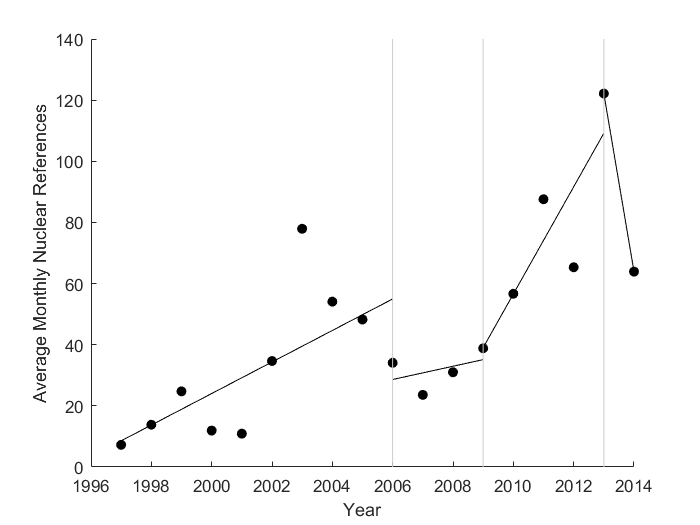
\includegraphics[width=0.7\linewidth]{../kcna_refs_updated}
	\caption{Monthly frequency of articles using the words ``nuke'' or ``nuclear'' were gathered from STALIN search results. Frequencies were averaged by year. Vertical lines represent years with nuclear tests, and slanted lines represent linear regressions on the years between tests.}
\label{fig:kcna_refs}
\end{figure}


At the end of 2011, Kim Jong-il died and his son succeeded him as ruler of the DPRK. At this time, there was also a dramatic increase in nuclear rhetoric in KCNA articles, perhaps in an attempt to reinforce the strength of the new regime in the eyes of the international community \cite{rich14}. This also did not directly feed into an escalatory cycle, although there were obviously a great deal of secondary impacts to the changeover of power.

\subsection{Results and Trends}

The clearest trend in North Korean nuclear rhetoric has been its dramatic increase over time. This is shown in figure \ref{fig:kcna_refs}, which tracks average monthly references for each year 1997-2014. In general, the data follow an upward trend and indeed the rate at which references increase also seems to be increasing---which tracks with the rise in distinct escalatory cycles as time passes. In general, it seems evident that the DPRK has been ramping up its nuclear ambitions, both in word and deed, at an ever-increasing rate as time passes.

The implications are concerning: the longer the status quo remains, the more emphasis will likely be placed on retaining nuclear competence, both rhetorically and materially. This is confirmed by historical examination - where earlier cycles contained agreements to roll back the DPRK's nuclear programs almost completely, it has been made clear in more recent years that this is no longer an option the DPRK will consider. All else being equal, the more time passes, the harder it may become to achieve the stated US objective of complete denuclearization.

The rhetoric used by North Korea to discuss nuclear tests and other significant military incidents suggests that such actions are, to a significant extent, posturing for the attention of the United States. This weakens justification for the emphasis many politicians place on returning to multilateral negotiations like the six-party talks. Each additional participant in negotiations adds a new set of demands and their own agenda to the mix, and if no commensurate benefit is seen from adding more voices to the conversation, the tradeoff may not be worthwhile. The modern US diplomatic strategy relies heavily upon pressure created by the international community, but it seems that the DPRK is uninterested in the international community's perspective on nuclear matters.


\section{American Rhetoric}
\subsection{Time-Invariant}

Bleiker \cite{bleiker} analyzed American policy with respect to the DPRK, focusing on the Clinton and Bush administrations. He found a systematic trend in the rhetoric and apparent worldview of American officials rooted in Cold War ideology - the notion of the ``rogue state''. Defined oppositionally to US interests, the ``rogue state'' is a foreign threat that must be thwarted at every turn. The intensity of the rhetoric couching this notion has ebbed and flowed, but the fundamental paradigm remains the same, and has been identified by many scholars \cite{bleiker,cumings,sigal,smith}.

Furthering this analysis, Smith suggests that most American politicians view North Korea as either ``mad'' or ``bad'' - in each case, fundamentally malicious, and either unknowable (``mad'', and therefore impossible to negotiate with) or devious (``bad'', and therefore morally repugnant to engage in diplomacy with). This split is evidenced by the dual focus in public statements regarding the DPRK on their instability and the grave threat they pose to the United States and its allies \cite{smith}. 

Another rhetorical factor that frequently escapes mention in analysis of this relationship is the nuclear posturing done by the United States. Ever since the 1950s, when the US violated a portion of the Korean Armistice Agreement to place nuclear weapons in South Korea, American policy has consistently erred on the side of nuclear grandstanding with respect to the DPRK \cite{cumings}. Indeed, in 1999 the DPRK had been the subject of more nuclear threats from the US than any other nation \cite{sigal}. Three years later, a leaked Defense Department report identified the nation as one of seven potential targets for nuclear strikes \cite{harnisch}.

North Korea has been intermittently labeled ``America's greatest security threat'' \cite{cumings} since at least the 1990s. In conjunction with the ``rogue state'' ideology and consistently aggressive nuclear posturing, this has framed the nature of US-DPRK diplomacy for the entire timeframe of interest with respect to the escalatory cycles.

\subsection{Time-Variant}

During the years leading up to and including cycle 1, American politicians did not seriously believe in the possibility of a diplomatic solution to the North Korean nuclear dilemma. Consequently, the prospect of negotiations was talked around and avoided, and the language of diplomacy was always heavily couched in threats \cite{sigal}.

During cycle 2, as the conflict between the US and the DPRK escalated, the former insisted upon ``crime-and-punishment''-style diplomacy \cite{bleiker}, a regime in which the DPRK would have to back down and admit wrongdoing to avoid serious negative repercussions. Former president Carter's back-channel negotiations took a different approach---encouraging cooperation and offering concessions in exchange for a rollback in the North Korean nuclear program \cite{sigal}.

In 1999, as cycle 3 was drawing to a close, a number of influential reports were published emphasizing the importance of a new, `integrated' negotiation strategy. The Perry report, commissioned by President Clinton, advised building upon previous success with the Agreed Framework and drawing down negative incentives in parallel---rejecting status quo pressure-first diplomacy as non-sustainable and vulnerable to collapse in future crises \cite{perry}. The Armitage report, compiled by a number of individuals from the H.W. Bush Department of Defense, also advised acknowledging the place of serious diplomatic negotiations as a tool for dealing with the DPRK. The Armitage report, however, was far more critical of the Agreed Framework, casting it as a necessary but insufficient step in pursuing disarmament, but stopping short of advocating its dissolution \cite{armitage}. Meanwhile, Republican voices in Congress put pressure on the Clinton administration to stick to and even toughen the status quo strategy of demanding results from the DPRK before sanction draw-down could even be considered \cite{harnisch}. 

The necessity of courting Congressional approval for US-DPRK negotiation strategies pushed American demands higher and higher as the Clinton era gave way to Bush. To complicate matters further, different messages were broadcast by various departments within the administration - while the State Department (influenced by Armitage, of the aforementioned report) broadcast willingness to treat with the DPRK in a cooperative manner, the Defense Department (led by Donald Rumsfeld, a long-time DPRK hard-liner \cite{rumsfeld}) publicly favored a more aggressive approach \cite{harnisch}.

In early 2002, George Bush's Axis of Evil speech was a mostly-accurate indicator of the broader state of American policy views towards the DPRK. Within a few months, the Defense Department's Nuclear Posture Review was leaked, which outlined a plan for a potential nuclear strike on North Korea \cite{npreview}. Additionally, both the Posture Review and the official National Security Strategy of that year emphasized the legitimacy of pre-emptive strikes against ``rogue states'' \cite{bleiker}, rhetoric that was echoed by Rumsfeld in news conferences that fall \cite{harnisch}.

Talks in North Korea in late 2002 devolved quickly to accusations of cheating on the Agreed Framework, initiating cycle 4. Diplomats from other nations reported that the American diplomatic team ``immediately started with accusations'', resisting efforts at negotiation \cite{bleiker}. When the Agreed Framework collapsed and North Korea withdrew from the NPT, the Bush administration made little more than a token effort to maintain their adherence to nonproliferation norms \cite{huntley}. Meanwhile, focus began to shift from bilateral engagement with the DPRK towards multilateral diplomacy and pressures, as the six-party talks began in late 2003 \cite{crs13}.

Bush's second inaugural address reinforced his administration's general preference for encouraging regime change in places like North Korea and avoiding diplomacy with dictators. Emphasis continued to fall on making sure nuclear weapons did not fall into the ``wrong'' hands, rather than opposing proliferation in the general case---indeed, in discussing the NPT conference in 2005, a high-ranking State Department official claimed it was unreasonable to suggest non-proliferation efforts by America when countries like North Korea existed \cite{huntley}.

During cycle 5, an apparent relaxing of the previous hard-line stance of ``complete, verifiable, and irreversible disarmament'' during negotiations in the fourth round of six-party talks did not last long \cite{huntley}. In early 2006, an updated National Security Strategy was released by the Bush administration, emphasizing ``proactive counterproliferation'' and democracy-building \cite{nss06}. And though this document touted the successes of the six-party talks, the beginnings of a return to dogmatism is already apparent in both the preemptive strike rhetoric and in the explicit mention of the DPRK as being in need of regime change \cite{nss06}.

The Obama administration began its relationship with North Korea with an eye towards more open diplomacy, echoing campaign sentiments suggesting ``willingness to engage with `rogue' governments'' \cite{crs13}. In stark contrast to the Bush administration's distaste for the NPT \cite{huntley}, Obama's focus on reducing the global nuclear threat informed a renewed focus on bringing North Korea into the fold of non-proliferation norms \cite{crs13}.

The Obama administration has described its perspective as one of ``strategic patience'' \cite{crs13}, though critics claim this is code for putting the North Korean nuclear issue on the back burner \cite{green}. The administration has continued to push for sanctions in response to incidents like the 2012 satellite launch, but the preconditions for negotiations have been reduced from ``complete, verifiable, and irreversible'' disarmament \cite{huntley} to ``commit[ing] to steps toward denuclearization'' \cite{crs13}.

Additionally, the Obama administration has followed the Bush lead with respect to multilateralism by pushing for a return to the six-party talks \cite{crs13}, and emphasizing a sanctions strategy palatable to all members of the UNSC \cite{green}. This has been paired with a high degree of coordination with South Korea, from an uptick in joint military exercises to near-identical focus in diplomatic engagements \cite{crs13}.

\subsection{Results and Trends}
There is a distinct evolution in American rhetorical strategies as time has passed, largely correlated with various presidential administrations. During the Clinton administration, ``rogue state'' labeling and outward hostility was combined with back-channel negotiations---perhaps seeking to preserve a sort of moral high ground while still reaping the benefits of a more conciliatory stance.

The Bush administration, by contrast, focused on acting as the world's policeman, replacing non-democratic governments with US-friendly democracies, and altering the country's nuclear agenda to make sure ``the right people'' had nuclear weapons. These combined to strengthen the ``rogue state'' rhetoric of the Clinton administration---going so far as to heavily imply that the radical reorganization of North Korean governmental structure would be preferable to as-is negotiation. Bilateral communication was eschewed in favor of multilateral talks and all-or-nothing ultimata.

The Obama administration expanded the multilateral focus introduced by Bush - though the six-party talks fell apart in 2008, more recent years have seen significant increases in coordination between the United States and regional allies on the DPRK question. Additionally, a new emphasis on non-proliferation norms has informed the rhetorical strategies surrounding international consensus-building. In terms of direct contact with North Korean officials, ``strategic patience'' has become the focus, and although concessions are still demanded as preconditions to productive talks, the language of such demands has been toned down dramatically.

Across administrations, the DPRK has consistently been portrayed as a ``rogue state'', as unpredictable as it is dangerous. This rhetoric informs the standard bargaining position: North Korea's willingness to engage in productive diplomacy cannot be trusted until it has met substantive preconditions. The degree to which these preconditions have been emphasized has changed from president to president, but the fundamental framework has remained. 

Interestingly, the standard bargaining position has often been subverted by back-channel negotiations and the words of some individuals within the executive branch more willing to entertain the notion of broader compromises. It seems likely that this discrepancy between public posturing and quieter action is informed at least somewhat by the need to appear responsive to public opinion; the American people tend to be displeased by the notion that their tax dollars are going towards appeasing oppressive regimes. Like the North Korea government, American politicians tend to speak in hard-line generalities in order to appear strong in their convictions, but can occasionally be induced to compromise behind closed doors.

\chapter{Diplomatic Evolution}

In order to understand the current negotiating positions of both the United States and North Korea, it is instructive to examine the history of the diplomatic postures of both countries over the past several decades. The historical and rhetorical analyses above each form an important component of the larger picture. Rhetorical analysis showed how the countries talked about what they did, while historical analysis identified the events triggering and being triggered by national positions. To tie these together, the evolution of positions themselves must be examined.

This section will use political administrations as breakpoints for analyzing diplomatic changes over time. The changes in priorities and negotiating strategies across different American presidential administrations are obvious. Shifts due to changes in North Korean leadership may be more difficult to identify, but there are still some notable patterns.

\section{Pre-1994}

The official American policy on North Korea under George H.W. Bush was one of ``strong engagement'', under which the DPRK would be allowed minimal access to nuclear material and steered heavily towards noronproliferation \cite{cerami}. This, in practice, translated to ``coercive diplomacy'' that relied far more heavily on coercion than diplomacy. Despite occasional forward steps, the administration did not seriously believe progress was possible through negotiation \cite{sigal}.

When Clinton took office, neither the official policy nor its implementation initially changed. Indeed, resumption of joint US-ROK war games (a policy decision made by the departing Bush) paired with dramatic rhetoric about the threat posed by North Korea followed quickly on the heels of Clinton's inauguration \cite{cumings}. During cycle 2, North Korean concerns about American meddling with the IAEA's inspection objectives combined with dismay over the military exercises to produce a climate of brinksmanship and hostility \cite{cumings}.

\section{Clinton and Kim Jong-il, 1994--2000}

\subsection{Development of the Agreed Framework}

From the American perspective, the DPRK was trying to evade its responsibilities pursuant to the IAEA. However, the DPRK felt that the IAEA's demands were unreasonably stringent, and worse, shaped by an American agenda to punish North Korea for insufficient deference \cite{cumings}. The DPRK withdrew from the IAEA and refused to allow inspectors into its nuclear facilities \cite{iaea09}.

Meanwhile, the death of Kim Il-sung meant that Kim Jong-il took power in the midst of a crisis, facing American threats of both economic sanctions and military power \cite{jun,cerami,cnn99}. The latter was particularly vexing to the new leader, for whom cancellation of war games the previous year had been a point of personal pride \cite{farrell}. The former also specifically coincided with a time of economic weakness and stagnation in the DPRK. The late days of Kim Il-sung's regime saw a slight but important opening of the North Korean economy to some foreign trade \cite{sigal}, which brought with it new avenues by which international pressure could be brought to bear.

While the DPRK would likely have come out on the bottom of a military engagement, this did not mean that war would serve American interests. The Yongbyon site could not be targeted without risking serious regional radiation release \cite{beal}. Even absent that concern, definitively crippling the North Korean nuclear program would require more confidence than US officials possessed that there were no nuclear sites that remained secret \cite{sigal}. Total war with North Korea would cost many thousands of lives---American, and North and South Korean---and was thus similarly unpalatable \cite{cumings}. Thus, though the military threat posed by the United States to the DPRK was serious (and came extremely close to realization \cite{cnn99}), it was not something American politicians wanted to do given any alternative.
	
The stage was set, therefore, for productive negotiation between the two parties. Both felt that they had been wronged by the way the other was interacting with the IAEA. The DPRK was backed into a corner, with a relatively untested leader facing serious threats to his nation that could no longer be averted by stonewalling. And the United States, also under new leadership, found the harsher methods in its diplomatic arsenal too risky \cite{hecker2}.

Though international pressure played a role in the crisis, the actual acts of diplomatic engagement were bilateral. This fits with empirical data suggesting that the DPRK's nuclear posture has always been primarily shaped by US-DPRK politics \cite{rich14}. The crisis was defused by the development of the Agreed Framework, negotiated with the aid of former president Jimmy Carter. This agreement, under which the DPRK froze its nuclear program in exchange for concrete guarantees of energy assistance \cite{agreed}, was very much in line with the goals of the first Bush administration's North Korea policy, which the Clinton administration made a point of continuing \cite{cerami} - although the methods of engagement employed in its negotiation were far more conciliatory than had previously been utilized \cite{sigal}.

\subsection{After the Agreed Framework}

Another diplomatic crisis emerged four years after the Agreed Framework was signed. It was initiated by a DPRK-claimed satellite launch that most onlookers viewed as a missile test---a dangerous leap forward in the path towards nuclear weapons \cite{orfall}. This was a major test of the diplomatic principles at play during Agreed Framework negotiations, not least because its implementation had been hindered by those same voices in Congress who initially opposed its negotiation \cite{hecker2}. Three months later, the United States offered sanction relief in exchange for termination of the DPRK missile program, but the DPRK argued that this sanction relief should already have occurred as part of the Agreed Framework and the fact that it had not yet was a failure on the part of the Americans \cite{davenport}. This argument was presumably referencing the Framework's mandate that both nations ``reduce barriers to trade and investment'' with the other within three months of signature \cite{agreed}, which had not been followed owing to earlier disputes regarding ballistic missiles \cite{davenport}.

The negotiation of this cycle coincided with the release of the Perry Report, which notably advocated for a change in American diplomatic attitude towards a stance that favored carrots as well as sticks \cite{perry}. Though the goal was still curtailing North Korean proliferation, this marked the apex of the softening attitude towards agreements seen under Clinton \cite{bleiker}. Indeed, cycle 3 concluded with the first agreement between the two countries under which the United States acknowledged North Korea's right to exist, and was immediately followed by talks between Kim Jong-il and the US Secretary of State \cite{hecker2}.
			
The Clinton era was thus marked by a ``coercive diplomacy'' that grew ever more willing to focus on the diplomacy side---at least within the Executive. Substantive action occurred in the form of negotiations resulting in serious agreements, but pushback from conservatives in Congress limited the efficacy of their implementation \cite{harnisch}. This was, perhaps, a sign of things to come once Bush took office.
	
\section{Bush and Kim Jong-il, 2001--2008}

\subsection{Collapse of the Agreed Framework}

From the outset, the Bush administration had a very different view of US-DPRK relations. Focus shifted away from non-proliferation as a universal good, and negotiation with unfriendly nations became a sign of unacceptable weakness \cite{bleiker}. Nowhere was this better exemplified than Bush's 2002 State of the Union speech, during which he identified North Korea as a member of an ``axis of evil'' supporting global terrorism \cite{sotu02}. This was shortly followed by a number of Defense Department documents emphasizing the legitimacy of preemptive nuclear strikes and other military actions against countries seeking weapons of mass destruction \cite{bleiker,npreview}.

As the US president and Defense Department ramped up hostile rhetoric against North Korea, the State Department still clung to Clinton-era negotiation \cite{harnisch,armitage}. This split between departments of the US government did little to improve the situation, producing confusion and mistrust in both the DPRK and regional American allies.

Meanwhile, the DPRK used Bush's ``axis of evil'' comments to justify a renewed focus on nuclear weapons development \cite{bleiker}. Discussion of nuclear matters in public North Korean media increased dramatically \cite{rich14}. With the United States on the record as mistrusting North Korea to the point of considering preemptive military action, production of nuclear weapons became an imperative for survival \cite{hecker2}.

In this environment, the first official visit by a senior American official under the Bush administration turned swiftly to disaster. The DPRK viewed the American group's attitude as ``high handed and arrogant'' \cite{kcna3}, and even Western diplomats present at the time agreed that the Americans immediately began with accusations \cite{bleiker}. The result was North Korea admitting to a secret uranium enrichment program, which set off the chain reaction of events comprising cycle 4: suspension of the Agreed Framework, withdrawal from the NPT, and expulsion of IAEA inspectors \cite{iaea09}. 

The collapse of these agreements, at face value a major blow to American interests in North Korea, suited the Bush agenda. The Agreed Framework had been a thorn in the side of the Bush administration, particularly in light of its provisions with respect to an LWR program and the base fact that it constituted a substantive agreement with an ``evil'' nation \cite{harnisch}. The DPRK's withdrawal from the NPT was irrelevant to an administration more concerned with cementing the military supremacy of the US and its allies than in maintaining global non-proliferation norms \cite{huntley}.

In sum, the Bush administration's preoccupation with black-and-white diplomatic morality and their desire to position the US as the world's policeman sounded a death knell for the progress previously made in US-DPRK relations. They primed North Korea with dramatically hostile rhetoric and barely-veiled threats, then used the resultant hostility as an excuse to cancel unwanted agreements while retaining the moral high ground.

Of course, this was enabled in large part by the fact that the DPRK did, in fact, pursue nuclear weapons and admitted to doing so when pressed. North Korea was a convenient moral scapegoat for the Bush administration, but it would not have become so absent its nuclear history and apparent ambitions. There is some possibility that they did not actually possess nuclear weapons at the time of this admission, since they only claimed to have \emph{pursued} them \cite{harnisch}, at which point their choice to reveal the program might suggest they also desired to rid themselves of the agreements, which restricted their nuclear development. 

\subsection{Rise of the Six-Party Talks}

Despite the Bush administration's evident hostility towards the concept of negotiating directly with North Korea, they were still verbally insistent that they hoped for and believed in a diplomatic solution \cite{bleiker}. The compromise seemed to come in the form of a renewed focus on multilateralism with the six-party talks. This model seemed well suited to the notion that increasing coercive pressure on North Korea would force them to come to the table on American terms. And though Bush did not exactly champion global non-proliferation norms, his administration was still perfectly willing to leverage the power of international coalitions to press the DPRK. This approach, however, proved far less effective than might be desired.

First, the six involved countries (China, Japan, both Koreas, Russia, and the US) came to the table with a wide array of incentives and goals. If the US intended to show North Korea that its behavior was unacceptable, it would first have to convince nations with complicated and frequently opposing priorities to present a unified front. Given that diplomats from most other parties pointed to American intractability as a major impediment to substantive progress \cite{park6pt}, trying to build a coalition around this position was a tall order indeed.

It seems implausible that the Bush administration could not predict that its dogmatic bargaining style would mesh poorly with the intricacies of multilateral diplomacy. Nor is it surprising that this exacerbated existing tensions between the desires of other members of the six-party talks. Given this, it is not unreasonable to conclude that the six-party talks were, if not set up for failure, at least not expected to succeed. They created an appearance of progress by bringing North Korea to talks without requiring the US to soften its position, a feat that could not have been accomplished in primarily bilateral diplomacy. This insulated the US from the consequences of its attitude by providing many alternate sources of blame when talks broke down.

Though the six-party talks were designed to bring the perspectives of all six nations to bear, the DPRK's focus on bilateral interactions with the United States \cite{rich14,park6pt} contributed heavily to their successes and failures. Cycle 5 demonstrated how unilateral American action taken to limit the DPRK's economic resources ground the six-party talks to a halt \cite{greenlees}, and reversal of that action during cycle 6 almost immediately preceded the talks' first action-oriented agreements \cite{js5,js6}. 

Once again, the Bush administration's distaste for letting ``evildoers'' benefit from its policies nearly scuppered substantive diplomacy when the US failed to follow through on promises to remove the DPRK from its State Sponsors of Terror list \cite{nti15}. The US only caved once the IAEA warned that North Korean fuel reprocessing was imminent \cite{iaea09}. Given the Bush administration's prior behavior, this is hardly surprising---it would have otherwise been difficult to imagine a president so focused on moral righteousness in American foreign policy making a symbolic move like removing a sworn enemy from a list identifying them as such.

Although the Bush administration's latter days contained more dialogue and fewer diatribes than they began with, all-or-nothing demands and foot-dragging on agreements were still the standard operating procedure. During this time, North Korea made serious advancements in its nuclear program and removed itself from international agreements intended to curb its progress. They began to conceptualize of their role in negotiations as one of an established nuclear power, rather than merely a country seeking nuclear technology \cite{hecker2}. However, they did continue to come to the table for negotiations---claiming repeatedly to be willing to make changes, but not without getting something in return. That last part perhaps best summarizes the conflict during this time period---the Bush administration wanted changes, but could not accept that making changes would require them to make concessions.

\section{Obama and Kim Jong-il, 2009--2011}

American policy towards North Korea once again underwent a radical shift under Obama, at least rhetorically. In his inaugural address, he emphasized willingness to engage in negotiations even with historic enemies \cite{obama}, and during his campaign he promised to focus on engagement with the DPRK \cite{delury}. These principles were tested early in Obama's first term with the events constituting cycle 7---including both a missile launch and a nuclear test.

The motivation for these actions may have been primarily political---a loss of patience on the North Korean side for waiting for the US to blink first. It is also likely, however, that scientific opportunism played a role---with a strong desire to improve their nuclear weapon technology and an interest in minimizing potential consequences, it made sense for the DPRK to conduct this testing while the Obama administration was still gathering its thoughts on foreign strategy \cite{hecker2}.

A third potential motivating factor was the perceived strength of the Kim regime. After rumors of Kim Jong-il's ill health circulated in late 2008, a show of military power like the missile test followed by escalation to a nuclear test may have been intended to shore up the North Korean leader's reputation \cite{hecker2}. KCNA coverage of this nuclear test focused more on the international community than it did specifically the United States (unlike other nuclear and non-nuclear military incidents) \cite{sin}. This suggests that the third explanation is at least more persuasive than the notion that Kim Jong-il was testing the waters of the Obama administration. Of course, the most mundane explanation---that the test occurred early in Obama's presidency because that happened to be when North Korea was first able to do the tests it wanted---is also plausible.

After cycle 7, US policy crystallized as a strategy of ``strategic patience'' \cite{crs13}, under which it was believed that the status quo would provide sufficient incentives for North Korea to initiate diplomatic interactions absent further American pressure \cite{snyder2}. This strategy relied upon the notion that existing sanctions and agreements would slow the growth of the North Korean nuclear program to the point where no serious breakthroughs could occur. Though the State Department under Obama disavowed the notion of continuity between their North Korea strategy and that of the Bush administration, the substantive differences between the two was perhaps less than might be inferred from their rhetoric \cite{delury}. The Bush administration extricated itself from most agreements related to the DPRK and only began halfhearted negotiations again relatively late. Meanwhile, the Obama administration made little more than token efforts to maintain the level of negotiations inherited from Bush, and mostly appeared to intend to leave North Korea to its own devices \cite{delury}.

While waiting for the DPRK to make the first move, American strategy also re-emphasized coordination with regional allies---while the stated objective was an eventual return to multilateral negotiations in the form of the six-party talks, the Obama administration oversaw a much greater degree of coordination between American diplomatic posture and that of South Korea and Japan than had occurred under Bush \cite{crs13,snyder2}. This kind of coordination could serve to mitigate some of the troubles that plagued previous rounds of talks, were they ever to resume.

On the other hand, linking American and South Korean diplomatic strategies tipped the scale back from ``strategic patience'' to aggressive action during the events of cycles 8 and 9---in line with the ROK, the US imposed sanctions on North Korea after the sinking of the Cheonan, and refocused on joint military exercises in the area \cite{starr}.

North Korean news coverage did its best to segregate the Cheonan and Yeonpyeong incidents from discussion of nuclear proliferation in an apparent attempt to maintain the status quo on nuclear matters \cite{rich12}. Unfortunately for the DPRK, international media made no similar attempts \cite{beal}, and the United States responded to the incidents with sanctions and an increased interest in cooperating with the hawkish policies at the fore of South Korean rhetoric \cite{crs13}.

In the months immediately prior to Kim Jong-il's death, the US began negotiating what would eventually become the Leap Day Agreement. The policy of ``strategic patience'' had clearly failed. In late 2010, DPRK officials had revealed a uranium enrichment and LWR program far more robust than the US expected to exist, revealing the American belief that the status quo would stop North Korean nuclear advancement to be flawed \cite{snyder2}. Response to the Yeonpyeong and Cheonan incidents had further suggested that sanctions were not significantly more productive than disengagement \cite{delury}. Once again, having exhausted all other options and still uninterested in direct military conflict, the United States turned to diplomacy.

\section{Obama and Kim Jong-un, 2012-2013}

Kim Jong-il's death briefly threw negotiations into turmoil \cite{crs13}---perhaps because the US was waiting to see if the transition to Kim Jong-un's leadership would cause the collapse that many experts had been forecasting for years \cite{delury}. This did not occur, however, and the DPRK suggested resumption of talks, after which an agreement was announced on February 29, 2012 \cite{delury}. The United States agreed to provide significant quantities of food aid in exchange for a moratorium on nuclear activities and the return of IAEA inspectors \cite{crs13}.

Though the United States hoped that the Leap Day Agreement would forestall further nuclear provocations by the DPRK, announcement of a satellite launch a mere three weeks later (the beginning of cycle 10) suggested that these hopes were in vain \cite{snyder2}. The DPRK insisted that these actions were an exercise of their right to peaceful space exploration \cite{crs13}, and claimed to still be interested in implementing the Agreement. However, the US (and the international community \cite{unsc13}) saw this action as a provocative missile test \cite{davenport}. This meant that, to American eyes, the Leap Day Agreement had collapsed and the diplomatic approach was judged a wholesale failure \cite{delury}.

Following this ``failure'', the US began to push for more aggressive UNSC sanctions than had been seen previously during the Obama administration, and continued this when another ``satellite launch'' occurred at the end of the year \cite{crs13}. The DPRK proceeded to conduct a nuclear test in early 2013, once again facing severe sanctions from the UNSC \cite{davenport}. Whether out of frustration with the Agreement's inability to change North Korean behavior or due to internal pressure from conservatives in Congress, the Obama administration once again swung from a more pro-dialogue stance to one in favor of punishment and sanctions \cite{snyder2}.
\chapter{Conclusions}

\section{The Agreed Framework and the Leap Day Agreement}

In tracing the history of American-North Korean nuclear diplomacy, it is worthwhile to compare the two major bilateral agreements between the nations - the Leap Day Agreement and the Agreed Framework. Though both ultimately collapsed, the differences in modes of failure are illustrative for the purposes of identifying successes and flaws in the American diplomatic model.

The Leap Day Agreement, like the Agreed Framework, promised aid from the United States in exchange for a freeze on the North Korean nuclear program. Unlike the Agreed Framework, which lasted for several years of spotty implementation only to peter out in the midst of a crisis, the Leap Day Agreement lasted less than a month. The difference was one of both circumstance and attitude.

The Agreed Framework took shape when both parties were actively seeking an escape from the escalatory cycle they were embroiled in. The DPRK was facing a flagging economy, strict international sanctions, and serious military threats from the United States. Meanwhile, the United States was unwilling to stomach the consequences of following through on the military threat, and was running out of options for producing economic pressure. Thus, both sides had strong incentives to cooperate with one another at least enough to weather the crisis.

During the negotiation of the Leap Day Agreement, however, the pressures felt by each party were far less symmetric. The DPRK was in a much stronger position than it had been in the 1990s. As a result of a decade mostly unfettered by the direct oversight of the international community (first due to Bush's aggressive disengagement from nonproliferation-focused agreements, then due to Obama's strategic patience), their nuclear program was robust enough that they no longer considered the American military an existential threat \cite{harnisch,hecker2}. Sanctions no longer seemed as effective a threat---perhaps because they were ``smart sanctions'' focused on weapons technology \cite{delury}, perhaps because the North Korean economy was in less dire straits, or perhaps because the international community was not following through on enforcing sanctions\cite{perlez}.

Meanwhile, the United States had come to the alarming conclusion that nothing else it tried had worked. ``Strategic patience'' relying on sanctions and other measures already in place seemed to have been based on a fundamental misestimation of the technical capacity of the North Korean nuclear program \cite{snyder2}. The sanctions didn't seem to be working, and the US was out of options---just like in 1994. This time, however, it was only American negotiators that were desperate.

The United States, then, placed a great deal of significance on the terms of the Leap Day Agreement, hoping strongly that it would succeed. The DPRK, on the other hand, was less concerned, which made them comfortable with pushing the boundaries of the Agreement. They took a sticking point from the Agreement's negotiations---whether satellite launches were legitimate enterprises or unacceptable tests of missile technology \cite{delury}---and demanded that their interpretation of the Agreement be accepted. They simultaneously affirmed willingness to hold up what they saw as their end of the bargain---the fact that they have previously shown no compunctions about declaring their departure from agreements suggests that this may even have been a sincere declaration.

Meanwhile, although the urgency of restraining the North Korean nuclear program would seem to have been a strong motivator in forcing the US to go to the bargaining table initially, it didn't seem to motivate them to attempt to salvage the Leap Day Agreement. Immediately upon the start of cycle 10, the US seemed to give up on the Agreement as a failure and indeed repudiated bilateral negotiations with the DPRK as a strategy wholesale \cite{delury}.

This may have been motivated by the belief that capitulating to North Korean interpretations of agreements would damage American credibility beyond repair---a view that seems to hold sway among conservative American politicians (who likely would have loudly criticized the Obama administration had any apparent capitulation occurred) and many of those involved in the UNSC sanctioning efforts. It seems bizarre to abandon the greatest opportunity in recent years to engage in actual negotiations over fear of diminished ability to negotiate. In general, however, this seems consistent with much of the Obama administration's tactics---in the interest of avoiding taking any diplomatic tools out of the toolbox permanently, many opportunities to actually use the tools as intended have been lost.

In sum, the Agreed Framework lasted longer than the Leap Day Agreement because there was more buy-in from both sides at the start. Likewise, the Agreed Framework collapsed as this buy-in eroded on both sides. This exacerbated the North Korean concerns about American intentions that informed their unwillingness to make the first move. North Korean reticence, in turn, reinforced the American view that North Korea wasn't to be trusted. The Leap Day Agreement seemed more necessary to the US than it did to the DPRK, so when the US claimed that North Korean action had invalidated the Agreement, the DPRK did not have especially strong incentives to fight the collapse.

\section{Lessons Learned and Future Prospects}

There have been circumstances during which it has been possible to get the DPRK to agree to dial back its nuclear program. There have even been circumstances in which it has actually done so. The difficulty lies in identifying common threads that tie these circumstances together, and in attempting to recreate them.

American strategy in the wake of the collapse of the Leap Day Agreement has two primary components. The first eschews direct contact with the DPRK - a vestige of the ``strategic patience'' of the early Obama days, or perhaps a reaction to the ``failure of diplomacy'' evidenced by the Agreement's collapse. The second emphasizes construction of international pressure - through both global nonproliferation norms and direct sanctions from the UNSC and other bodies.

This bifurcated strategy seems at odds with the lessons of the historic record. Negative international pressure spearheaded by the United States has a notably poor track record, and the crises of the first four years of Obama's presidency highlighted the dangers of disengaging and leaving North Korea to its own devices.

\subsection{The Problem With International Pressure}

For North Korea to come to the table with denuclearizing intentions, it must feel vulnerable - pressured by both external and internal forces. The international community is sometimes a useful tool in creating this pressure, as demonstrated by the sanctions before the Agreed Framework and the brief success of the six-party talks' statements of principles. 

However, too much apparent curation of international pressure by the United States risks inciting anger from the DPRK, which is always vigilant for American conspiracies forcing it to act in certain ways. If the DPRK suspects collusion between the US and NGOs or countries involved in nuclear talks or implementation of agreements, it tends to balk, doubling down on escalatory behavior and inflammatory rhetoric to avoid what it sees as American imperialism. Thus, even though the existence of external pressure may encourage the DPRK to negotiate, cultivating this pressure in a productive manner is extremely difficult.

\subsection{The Problem With Strategic Patience}

If the DPRK was sufficiently hindered in development of nuclear and missile technology by the existence of safeguards, oversight, and existing sanctions, a policy putting the onus on North Korea to act first might work. However, that was not the case in 2009 and it has not been the case since then. North Korea has become more motivated and confident in its nuclear program with every passing year---and, with that, the chance of total denuclearization becomes more and more remote.

First, from a practical and ideological standpoint, the further North Korea progresses on its nuclear program, the less likely it is to want to denuclearize. A program in relative infancy would be relatively easy to shut down. A program with facilities capturing much of the weapons supply chain and with a number of successful tests under its belt, however, involves far more investment and as such would be commensurately harder to shutter. Greater material incentives would be necessary to offset the increased financial loss represented by closure. Also, if the DPRK's national image has been tied to the success of its program, the difficulty of convincing it to shut down the program increases substantially. This latter factor in particular has been noticeable in the DPRK's posture over time \cite{rich14,hecker2}.

Second, the gap between how much trust exists within the US-DPRK relationship and how much is necessary for denuclearization to work increases as the North Korean program advances. A more robust nuclear program means more facilities, more materials, and more missiles - and with this increase in numbers comes increased complexity for monitoring and drawdown efforts. Verification that complete denuclearization has occurred is a difficult problem even when all parties have a reasonable working relationship. As years pass and US-DPRK interactions continue to show suspicion or bad faith, the likelihood of a relationship in which denuclearization can be believed decreases as well.

Waiting for the DPRK to make the first move, then, is both theoretically unsound and contraindicated by historical facts. The DPRK is not under sufficient existential pressure to foster willingness to talk on American terms, and as long as the status quo persists, this means they will continue to advance their nuclear program - which will itself make future negotiations on denuclearizing terms less feasible.

\subsection{Is American Strategy Reasonable?}

Current American strategy is bifurcated between indirect engagement (through cultivating pressure via the international community) and direct disengagement (through unwillingness to make the first diplomatic overture). This is informed to some extent by historical facts---the DPRK has come to the bargaining table when it has felt sufficient pressure, and does seem more willing to stick to agreements for longer if it is the initiating party in negotiations. However, the conditions in the status quo are sufficiently far from the conditions under which these strategies have succeeded that they no longer seem likely to work.

The particular brand of pressure engendered by American advocacy of tough measures like increased UNSC sanctions is highly likely to make the DPRK double down on hard-line stances in order to prove it will not be bullied. The North Korean nuclear program is both robust and significantly linked with the nation's self-perception of international legitimacy. The only hope, then, would be to create sanctions that pose a sufficient existential threat to the DPRK that it has no choice but to negotiate - a level which, through accident or concern for civilian life, the UNSC has not reached\footnote{Perhaps some internal catastrophe, like a series of natural disasters or the sudden death of Kim Jong-un could also produce such an existential threat, but aside from assassinations or the deliberate triggering of a volcanic eruption, this is beyond the ability of the United States to affect.}. 

This indicates that current American strategy - and, in particular, focus on extracting commitments to complete denuclearization before further talks can occur---is fundamentally flawed. Indeed, even if the precondition were dispensed with, it is hard to imagine a scenario in which the DPRK would seriously commit to abandoning its nuclear ambitions without dramatic shifts to the status quo. America must either radically reconsider what it is willing to do in order to remove North Korea as a nuclear threat, or face the reality that the DPRK is a nuclear power and shift its focus to damage control.
%\appendix
%\chapter{Code Used to Recover Data from STALIN Results}

\begin{verbatim}

//sets up arrays to store annual averages
dateRangeLength = barchartBody.length-2;
arrayYears = Array(dateRangeLength-1);
arrayRefs = Array(dateRangeLength-1);


//iterates from 1997-2014 because those are all the years with
// complete info available
for (i = 1; i<dateRangeLength; i++){
    numRefs = 0;
    numMonths = 0;
    for (j = 0; j<barchartBody[i].rows.length; j++){
    //the first item for each year contains year, month, and bar.
    //everything subsequent does not contain year. so we have to test!
        if (j==0){
            numRefs += dealWithZerosWell(barchartBody[i].rows[j].cells[2].
                             firstChild.nextSibling.firstChild.nextSibling.
                             innerHTML);
        }
        else{
            numRefs += dealWithZerosWell(dealWithZerosWell(barchartBody[i].rows[j].
                            cells[1].firstChild.nextSibling.
                            firstChild.nextSibling.innerHTML));
        }
    numMonths++;
    }
	
avgRefs = numRefs/numMonths;
year = i+1996;

//prints values for this iteration to the console
console.log("the year is " + year);
console.log("avg refs are " + avgRefs);

//saves values for this iteration into the array
arrayYears[i-1]=year;
arrayRefs[i-1]=avgRefs;
}

/*
The STALIN author decided to represent 0 frequency with a blank space. Let's make sure that saves properly.
*/
function dealWithZerosWell(testVal){
    if (Number.isNaN(testVal)){
        return 0;
    }
    return parseInt(testVal);
}
\end{verbatim}

\clearpage
\newpage

%\chapter{Figures}

\vspace*{-3in}

\begin{figure}
\vspace{2.4in}
\caption{Armadillo slaying lawyer.}
\label{arm:fig1}
\end{figure}
\clearpage
\newpage

\begin{figure}
\vspace{2.4in}
\caption{Armadillo eradicating national debt.}
\label{arm:fig2}
\end{figure}
\clearpage
\newpage

%% This defines the bibliography file (main.bib) and the bibliography style.
%% If you want to create a bibliography file by hand, change the contents of
%% this file to a `thebibliography' environment.  For more information 
%% see section 4.3 of the LaTeX manual.
\begin{singlespace}
\bibliography{main}
\bibliographystyle{ieeetr}
\end{singlespace}

\end{document}

